\documentclass[1p]{elsarticle_modified}
%\bibliographystyle{elsarticle-num}

%\usepackage[colorlinks]{hyperref}
%\usepackage{abbrmath_seonhwa} %\Abb, \Ascr, \Acal ,\Abf, \Afrak
\usepackage{amsfonts}
\usepackage{amssymb}
\usepackage{amsmath}
\usepackage{amsthm}
\usepackage{scalefnt}
\usepackage{amsbsy}
\usepackage{kotex}
\usepackage{caption}
\usepackage{subfig}
\usepackage{color}
\usepackage{graphicx}
\usepackage{xcolor} %% white, black, red, green, blue, cyan, magenta, yellow
\usepackage{float}
\usepackage{setspace}
\usepackage{hyperref}

\usepackage{tikz}
\usetikzlibrary{arrows}

\usepackage{multirow}
\usepackage{array} % fixed length table
\usepackage{hhline}

%%%%%%%%%%%%%%%%%%%%%
\makeatletter
\renewcommand*\env@matrix[1][\arraystretch]{%
	\edef\arraystretch{#1}%
	\hskip -\arraycolsep
	\let\@ifnextchar\new@ifnextchar
	\array{*\c@MaxMatrixCols c}}
\makeatother %https://tex.stackexchange.com/questions/14071/how-can-i-increase-the-line-spacing-in-a-matrix
%%%%%%%%%%%%%%%

\usepackage[normalem]{ulem}

\newcommand{\msout}[1]{\ifmmode\text{\sout{\ensuremath{#1}}}\else\sout{#1}\fi}
%SOURCE: \msout is \stkout macro in https://tex.stackexchange.com/questions/20609/strikeout-in-math-mode

\newcommand{\cancel}[1]{
	\ifmmode
	{\color{red}\msout{#1}}
	\else
	{\color{red}\sout{#1}}
	\fi
}

\newcommand{\add}[1]{
	{\color{blue}\uwave{#1}}
}

\newcommand{\replace}[2]{
	\ifmmode
	{\color{red}\msout{#1}}{\color{blue}\uwave{#2}}
	\else
	{\color{red}\sout{#1}}{\color{blue}\uwave{#2}}
	\fi
}

\newcommand{\Sol}{\mathcal{S}} %segment
\newcommand{\D}{D} %diagram
\newcommand{\A}{\mathcal{A}} %arc


%%%%%%%%%%%%%%%%%%%%%%%%%%%%%5 test

\def\sl{\operatorname{\textup{SL}}(2,\Cbb)}
\def\psl{\operatorname{\textup{PSL}}(2,\Cbb)}
\def\quan{\mkern 1mu \triangleright \mkern 1mu}

\theoremstyle{definition}
\newtheorem{thm}{Theorem}[section]
\newtheorem{prop}[thm]{Proposition}
\newtheorem{lem}[thm]{Lemma}
\newtheorem{ques}[thm]{Question}
\newtheorem{cor}[thm]{Corollary}
\newtheorem{defn}[thm]{Definition}
\newtheorem{exam}[thm]{Example}
\newtheorem{rmk}[thm]{Remark}
\newtheorem{alg}[thm]{Algorithm}

\newcommand{\I}{\sqrt{-1}}
\begin{document}

%\begin{frontmatter}
%
%\title{Boundary parabolic representations of knots up to 8 crossings}
%
%%% Group authors per affiliation:
%\author{Yunhi Cho} 
%\address{Department of Mathematics, University of Seoul, Seoul, Korea}
%\ead{yhcho@uos.ac.kr}
%
%
%\author{Seonhwa Kim} %\fnref{s_kim}}
%\address{Center for Geometry and Physics, Institute for Basic Science, Pohang, 37673, Korea}
%\ead{ryeona17@ibs.re.kr}
%
%\author{Hyuk Kim}
%\address{Department of Mathematical Sciences, Seoul National University, Seoul 08826, Korea}
%\ead{hyukkim@snu.ac.kr}
%
%\author{Seokbeom Yoon}
%\address{Department of Mathematical Sciences, Seoul National University, Seoul, 08826,  Korea}
%\ead{sbyoon15@snu.ac.kr}
%
%\begin{abstract}
%We find all boundary parabolic representation of knots up to 8 crossings.
%
%\end{abstract}
%\begin{keyword}
%    \MSC[2010] 57M25 
%\end{keyword}
%
%\end{frontmatter}

%\linenumbers
%\tableofcontents
%
\newcommand\colored[1]{\textcolor{white}{\rule[-0.35ex]{0.8em}{1.4ex}}\kern-0.8em\color{red} #1}%
%\newcommand\colored[1]{\textcolor{white}{ #1}\kern-2.17ex	\textcolor{white}{ #1}\kern-1.81ex	\textcolor{white}{ #1}\kern-2.15ex\color{red}#1	}

{\Large $\underline{11a_{88}~(K11a_{88})}$}

\setlength{\tabcolsep}{10pt}
\renewcommand{\arraystretch}{1.6}
\vspace{1cm}\begin{tabular}{m{100pt}>{\centering\arraybackslash}m{274pt}}
\multirow{5}{120pt}{
	\centering
	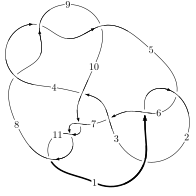
\includegraphics[width=112pt]{../../../GIT/diagram.site/Diagrams/png/337_11a_88.png}\\
\ \ \ A knot diagram\footnotemark}&
\allowdisplaybreaks
\textbf{Linearized knot diagam} \\
\cline{2-2}
 &
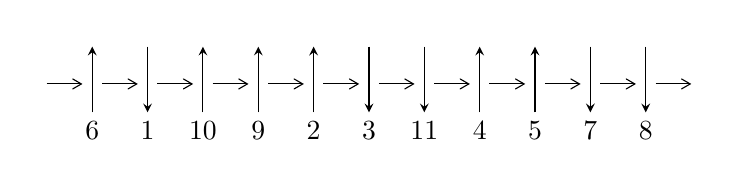
\begin{tikzpicture}[x=20pt, y=17pt]
	% nodes
	\node (C0) at (0, 0) {};
	\node (C1) at (1, 0) {};
	\node (C1U) at (1, +1) {};
	\node (C1D) at (1, -1) {6};

	\node (C2) at (2, 0) {};
	\node (C2U) at (2, +1) {};
	\node (C2D) at (2, -1) {1};

	\node (C3) at (3, 0) {};
	\node (C3U) at (3, +1) {};
	\node (C3D) at (3, -1) {10};

	\node (C4) at (4, 0) {};
	\node (C4U) at (4, +1) {};
	\node (C4D) at (4, -1) {9};

	\node (C5) at (5, 0) {};
	\node (C5U) at (5, +1) {};
	\node (C5D) at (5, -1) {2};

	\node (C6) at (6, 0) {};
	\node (C6U) at (6, +1) {};
	\node (C6D) at (6, -1) {3};

	\node (C7) at (7, 0) {};
	\node (C7U) at (7, +1) {};
	\node (C7D) at (7, -1) {11};

	\node (C8) at (8, 0) {};
	\node (C8U) at (8, +1) {};
	\node (C8D) at (8, -1) {4};

	\node (C9) at (9, 0) {};
	\node (C9U) at (9, +1) {};
	\node (C9D) at (9, -1) {5};

	\node (C10) at (10, 0) {};
	\node (C10U) at (10, +1) {};
	\node (C10D) at (10, -1) {7};

	\node (C11) at (11, 0) {};
	\node (C11U) at (11, +1) {};
	\node (C11D) at (11, -1) {8};
	\node (C12) at (12, 0) {};

	% arrows
	\draw[->,>={angle 60}]
	(C0) edge (C1) (C1) edge (C2) (C2) edge (C3) (C3) edge (C4) (C4) edge (C5) (C5) edge (C6) (C6) edge (C7) (C7) edge (C8) (C8) edge (C9) (C9) edge (C10) (C10) edge (C11) (C11) edge (C12) ;	\draw[->,>=stealth]
	(C1D) edge (C1U) (C2U) edge (C2D) (C3D) edge (C3U) (C4D) edge (C4U) (C5D) edge (C5U) (C6U) edge (C6D) (C7U) edge (C7D) (C8D) edge (C8U) (C9D) edge (C9U) (C10U) edge (C10D) (C11U) edge (C11D) ;
	\end{tikzpicture} \\
\hhline{~~} \\& 
\textbf{Solving Sequence} \\ \cline{2-2} 
 &
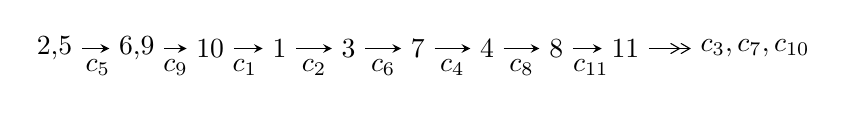
\begin{tikzpicture}[x=25pt, y=7pt]
	% node
	\node (A0) at (-1/8, 0) {2,5};
	\node (A1) at (17/16, 0) {6,9};
	\node (A2) at (17/8, 0) {10};
	\node (A3) at (25/8, 0) {1};
	\node (A4) at (33/8, 0) {3};
	\node (A5) at (41/8, 0) {7};
	\node (A6) at (49/8, 0) {4};
	\node (A7) at (57/8, 0) {8};
	\node (A8) at (65/8, 0) {11};
	\node (C1) at (1/2, -1) {$c_{5}$};
	\node (C2) at (13/8, -1) {$c_{9}$};
	\node (C3) at (21/8, -1) {$c_{1}$};
	\node (C4) at (29/8, -1) {$c_{2}$};
	\node (C5) at (37/8, -1) {$c_{6}$};
	\node (C6) at (45/8, -1) {$c_{4}$};
	\node (C7) at (53/8, -1) {$c_{8}$};
	\node (C8) at (61/8, -1) {$c_{11}$};
	\node (A9) at (10, 0) {$c_{3},c_{7},c_{10}$};

	% edge
	\draw[->,>=stealth]	
	(A0) edge (A1) (A1) edge (A2) (A2) edge (A3) (A3) edge (A4) (A4) edge (A5) (A5) edge (A6) (A6) edge (A7) (A7) edge (A8) ;
	\draw[->>,>={angle 60}]	
	(A8) edge (A9);
\end{tikzpicture} \\ 

\end{tabular} \\

\footnotetext{
The image of knot diagram is generated by the software ``\textbf{Draw programme}" developed by Andrew Bartholomew(\url{http://www.layer8.co.uk/maths/draw/index.htm\#Running-draw}), where we modified some parts for our purpose(\url{https://github.com/CATsTAILs/LinksPainter}).
}\phantom \\ \newline 
\centering \textbf{Ideals for irreducible components\footnotemark of $X_{\text{par}}$} 
 
\begin{align*}
I^u_{1}&=\langle 
3.81735\times10^{18} u^{55}-3.41298\times10^{18} u^{54}+\cdots+7.25836\times10^{18} b-6.54872\times10^{18},\\
\phantom{I^u_{1}}&\phantom{= \langle  }8.54661\times10^{18} u^{55}-1.96112\times10^{19} u^{54}+\cdots+7.25836\times10^{18} a-6.19813\times10^{18},\;u^{56}-2 u^{55}+\cdots-2 u+1\rangle \\
I^u_{2}&=\langle 
- a u+3 b+a+2 u+1,\;a^2+2 a u-7 u-7,\;u^2+u+1\rangle \\
I^u_{3}&=\langle 
b,\;a+u,\;u^2- u+1\rangle \\
\\
\end{align*}
\raggedright * 3 irreducible components of $\dim_{\mathbb{C}}=0$, with total 62 representations.\\
\footnotetext{All coefficients of polynomials are rational numbers. But the coefficients are sometimes approximated in decimal forms when there is not enough margin.}
\newpage
\renewcommand{\arraystretch}{1}
\centering \section*{I. $I^u_{1}= \langle 3.82\times10^{18} u^{55}-3.41\times10^{18} u^{54}+\cdots+7.26\times10^{18} b-6.55\times10^{18},\;8.55\times10^{18} u^{55}-1.96\times10^{19} u^{54}+\cdots+7.26\times10^{18} a-6.20\times10^{18},\;u^{56}-2 u^{55}+\cdots-2 u+1 \rangle$}
\flushleft \textbf{(i) Arc colorings}\\
\begin{tabular}{m{7pt} m{180pt} m{7pt} m{180pt} }
\flushright $a_{2}=$&$\begin{pmatrix}0\\u\end{pmatrix}$ \\
\flushright $a_{5}=$&$\begin{pmatrix}1\\0\end{pmatrix}$ \\
\flushright $a_{6}=$&$\begin{pmatrix}1\\- u^2\end{pmatrix}$ \\
\flushright $a_{9}=$&$\begin{pmatrix}-1.17748 u^{55}+2.70188 u^{54}+\cdots-7.40789 u+0.853930\\-0.525924 u^{55}+0.470213 u^{54}+\cdots+0.327275 u+0.902232\end{pmatrix}$ \\
\flushright $a_{10}=$&$\begin{pmatrix}-1.70341 u^{55}+3.17209 u^{54}+\cdots-7.08061 u+1.75616\\-0.525924 u^{55}+0.470213 u^{54}+\cdots+0.327275 u+0.902232\end{pmatrix}$ \\
\flushright $a_{1}=$&$\begin{pmatrix}- u\\u^3+u\end{pmatrix}$ \\
\flushright $a_{3}=$&$\begin{pmatrix}- u^3\\u^5+u^3+u\end{pmatrix}$ \\
\flushright $a_{7}=$&$\begin{pmatrix}- u^6- u^4+1\\u^8+2 u^6+2 u^4\end{pmatrix}$ \\
\flushright $a_{4}=$&$\begin{pmatrix}-0.0147560 u^{55}+0.313638 u^{54}+\cdots-6.67639 u+0.916847\\0.352209 u^{55}-0.918697 u^{54}+\cdots+1.18445 u+1.11145\end{pmatrix}$ \\
\flushright $a_{8}=$&$\begin{pmatrix}1.10278 u^{55}-2.44048 u^{54}+\cdots+5.22670 u-1.38381\\0.449311 u^{55}-0.0110571 u^{54}+\cdots+0.457669 u-0.899349\end{pmatrix}$ \\
\flushright $a_{11}=$&$\begin{pmatrix}-1.33623 u^{55}+3.16841 u^{54}+\cdots-7.38742 u+1.20484\\-0.480366 u^{55}+0.160009 u^{54}+\cdots+0.210912 u+0.917813\end{pmatrix}$\\ \flushright $a_{11}=$&$\begin{pmatrix}-1.33623 u^{55}+3.16841 u^{54}+\cdots-7.38742 u+1.20484\\-0.480366 u^{55}+0.160009 u^{54}+\cdots+0.210912 u+0.917813\end{pmatrix}$\\&\end{tabular}
\flushleft \textbf{(ii) Obstruction class $= -1$}\\~\\
\flushleft \textbf{(iii) Cusp Shapes $= -\frac{10988692710744958139}{3629180684127117001} u^{55}+\frac{21985136905178948607}{3629180684127117001} u^{54}+\cdots-\frac{18377034251590244150}{3629180684127117001} u+\frac{18266861748021250925}{3629180684127117001}$}\\~\\
\newpage\renewcommand{\arraystretch}{1}
\flushleft \textbf{(iv) u-Polynomials at the component}\newline \\
\begin{tabular}{m{50pt}|m{274pt}}
Crossings & \hspace{64pt}u-Polynomials at each crossing \\
\hline $$\begin{aligned}c_{1},c_{5}\end{aligned}$$&$\begin{aligned}
&u^{56}-2 u^{55}+\cdots-2 u+1
\end{aligned}$\\
\hline $$\begin{aligned}c_{2}\end{aligned}$$&$\begin{aligned}
&u^{56}+28 u^{55}+\cdots+4 u+1
\end{aligned}$\\
\hline $$\begin{aligned}c_{3}\end{aligned}$$&$\begin{aligned}
&u^{56}-3 u^{55}+\cdots+276 u+172
\end{aligned}$\\
\hline $$\begin{aligned}c_{4},c_{8},c_{9}\end{aligned}$$&$\begin{aligned}
&u^{56}+u^{55}+\cdots+12 u+4
\end{aligned}$\\
\hline $$\begin{aligned}c_{6}\end{aligned}$$&$\begin{aligned}
&u^{56}+2 u^{55}+\cdots+1554 u+481
\end{aligned}$\\
\hline $$\begin{aligned}c_{7},c_{10},c_{11}\end{aligned}$$&$\begin{aligned}
&u^{56}+3 u^{55}+\cdots-31 u+7
\end{aligned}$\\
\hline
\end{tabular}\\~\\
\newpage\renewcommand{\arraystretch}{1}
\flushleft \textbf{(v) Riley Polynomials at the component}\newline \\
\begin{tabular}{m{50pt}|m{274pt}}
Crossings & \hspace{64pt}Riley Polynomials at each crossing \\
\hline $$\begin{aligned}c_{1},c_{5}\end{aligned}$$&$\begin{aligned}
&y^{56}+28 y^{55}+\cdots+4 y+1
\end{aligned}$\\
\hline $$\begin{aligned}c_{2}\end{aligned}$$&$\begin{aligned}
&y^{56}+4 y^{55}+\cdots+28 y+1
\end{aligned}$\\
\hline $$\begin{aligned}c_{3}\end{aligned}$$&$\begin{aligned}
&y^{56}+9 y^{55}+\cdots+99952 y+29584
\end{aligned}$\\
\hline $$\begin{aligned}c_{4},c_{8},c_{9}\end{aligned}$$&$\begin{aligned}
&y^{56}-51 y^{55}+\cdots+48 y+16
\end{aligned}$\\
\hline $$\begin{aligned}c_{6}\end{aligned}$$&$\begin{aligned}
&y^{56}-20 y^{55}+\cdots-456284 y+231361
\end{aligned}$\\
\hline $$\begin{aligned}c_{7},c_{10},c_{11}\end{aligned}$$&$\begin{aligned}
&y^{56}-53 y^{55}+\cdots+747 y+49
\end{aligned}$\\
\hline
\end{tabular}\\~\\
\newpage\flushleft \textbf{(vi) Complex Volumes and Cusp Shapes}
$$\begin{array}{c|c|c}  
\text{Solutions to }I^u_{1}& \I (\text{vol} + \sqrt{-1}CS) & \text{Cusp shape}\\
 \hline 
\begin{aligned}
u &= -0.761612 + 0.706746 I \\
a &= -2.61065 - 0.67242 I \\
b &= \phantom{-}1.324630 - 0.244844 I\end{aligned}
 & \phantom{-}1.58146 - 5.73177 I & \phantom{-}1.83404 + 5.79402 I \\ \hline\begin{aligned}
u &= -0.761612 - 0.706746 I \\
a &= -2.61065 + 0.67242 I \\
b &= \phantom{-}1.324630 + 0.244844 I\end{aligned}
 & \phantom{-}1.58146 + 5.73177 I & \phantom{-}1.83404 - 5.79402 I \\ \hline\begin{aligned}
u &= \phantom{-}0.690346 + 0.801960 I \\
a &= \phantom{-}0.481692 + 0.412002 I \\
b &= -0.066092 - 0.603875 I\end{aligned}
 & -2.82580 + 2.62743 I & -4.75305 - 4.09062 I \\ \hline\begin{aligned}
u &= \phantom{-}0.690346 - 0.801960 I \\
a &= \phantom{-}0.481692 - 0.412002 I \\
b &= -0.066092 + 0.603875 I\end{aligned}
 & -2.82580 - 2.62743 I & -4.75305 + 4.09062 I \\ \hline\begin{aligned}
u &= \phantom{-}0.451244 + 0.989156 I \\
a &= \phantom{-}0.050142 - 0.437553 I \\
b &= -0.542520 + 0.123434 I\end{aligned}
 & -0.57122 + 2.77824 I & \phantom{-}2.95589 - 4.20688 I \\ \hline\begin{aligned}
u &= \phantom{-}0.451244 - 0.989156 I \\
a &= \phantom{-}0.050142 + 0.437553 I \\
b &= -0.542520 - 0.123434 I\end{aligned}
 & -0.57122 - 2.77824 I & \phantom{-}2.95589 + 4.20688 I \\ \hline\begin{aligned}
u &= \phantom{-}0.853869 + 0.316506 I \\
a &= -2.36674 - 0.45164 I \\
b &= \phantom{-}1.40459 - 0.32683 I\end{aligned}
 & -0.70521 - 8.81361 I & \phantom{-}1.89048 + 4.78995 I \\ \hline\begin{aligned}
u &= \phantom{-}0.853869 - 0.316506 I \\
a &= -2.36674 + 0.45164 I \\
b &= \phantom{-}1.40459 + 0.32683 I\end{aligned}
 & -0.70521 + 8.81361 I & \phantom{-}1.89048 - 4.78995 I \\ \hline\begin{aligned}
u &= -0.569045 + 0.945562 I \\
a &= -2.02662 - 1.07884 I \\
b &= \phantom{-}1.411350 + 0.084042 I\end{aligned}
 & \phantom{-}5.37458 - 1.80246 I & \phantom{-}7.34576 + 2.56666 I \\ \hline\begin{aligned}
u &= -0.569045 - 0.945562 I \\
a &= -2.02662 + 1.07884 I \\
b &= \phantom{-}1.411350 - 0.084042 I\end{aligned}
 & \phantom{-}5.37458 + 1.80246 I & \phantom{-}7.34576 - 2.56666 I\\
 \hline 
 \end{array}$$\newpage$$\begin{array}{c|c|c}  
\text{Solutions to }I^u_{1}& \I (\text{vol} + \sqrt{-1}CS) & \text{Cusp shape}\\
 \hline 
\begin{aligned}
u &= -0.631832 + 0.630832 I \\
a &= \phantom{-}2.75595 + 1.02264 I \\
b &= -1.399300 + 0.140066 I\end{aligned}
 & \phantom{-}6.29507 - 2.91322 I & \phantom{-}8.51117 + 4.03861 I \\ \hline\begin{aligned}
u &= -0.631832 - 0.630832 I \\
a &= \phantom{-}2.75595 - 1.02264 I \\
b &= -1.399300 - 0.140066 I\end{aligned}
 & \phantom{-}6.29507 + 2.91322 I & \phantom{-}8.51117 - 4.03861 I \\ \hline\begin{aligned}
u &= -0.829870 + 0.241336 I \\
a &= \phantom{-}0.509900 + 0.334719 I \\
b &= -0.240288 - 0.794736 I\end{aligned}
 & -5.93188 + 4.75475 I & -2.47991 - 3.65893 I \\ \hline\begin{aligned}
u &= -0.829870 - 0.241336 I \\
a &= \phantom{-}0.509900 - 0.334719 I \\
b &= -0.240288 + 0.794736 I\end{aligned}
 & -5.93188 - 4.75475 I & -2.47991 + 3.65893 I \\ \hline\begin{aligned}
u &= \phantom{-}0.374837 + 1.075050 I \\
a &= -0.490885 - 0.409888 I \\
b &= -1.087140 + 0.111404 I\end{aligned}
 & -0.27332 + 2.70620 I & \phantom{-0.000000 } 0 \\ \hline\begin{aligned}
u &= \phantom{-}0.374837 - 1.075050 I \\
a &= -0.490885 + 0.409888 I \\
b &= -1.087140 - 0.111404 I\end{aligned}
 & -0.27332 - 2.70620 I & \phantom{-0.000000 } 0 \\ \hline\begin{aligned}
u &= \phantom{-}0.268445 + 1.111910 I \\
a &= \phantom{-}0.146715 - 0.451206 I \\
b &= \phantom{-}1.272610 - 0.252980 I\end{aligned}
 & \phantom{-}0.50238 - 1.98879 I & \phantom{-0.000000 } 0 \\ \hline\begin{aligned}
u &= \phantom{-}0.268445 - 1.111910 I \\
a &= \phantom{-}0.146715 + 0.451206 I \\
b &= \phantom{-}1.272610 + 0.252980 I\end{aligned}
 & \phantom{-}0.50238 + 1.98879 I & \phantom{-0.000000 } 0 \\ \hline\begin{aligned}
u &= -0.385295 + 1.082820 I \\
a &= -0.468644 - 1.033150 I \\
b &= -0.004875 - 0.663333 I\end{aligned}
 & -3.45328 - 1.33657 I & \phantom{-0.000000 } 0 \\ \hline\begin{aligned}
u &= -0.385295 - 1.082820 I \\
a &= -0.468644 + 1.033150 I \\
b &= -0.004875 + 0.663333 I\end{aligned}
 & -3.45328 + 1.33657 I & \phantom{-0.000000 } 0\\
 \hline 
 \end{array}$$\newpage$$\begin{array}{c|c|c}  
\text{Solutions to }I^u_{1}& \I (\text{vol} + \sqrt{-1}CS) & \text{Cusp shape}\\
 \hline 
\begin{aligned}
u &= -0.698151 + 0.927977 I \\
a &= \phantom{-}1.99746 + 0.91434 I \\
b &= -1.275360 - 0.207940 I\end{aligned}
 & \phantom{-}0.926044 + 0.238949 I & \phantom{-0.000000 } 0 \\ \hline\begin{aligned}
u &= -0.698151 - 0.927977 I \\
a &= \phantom{-}1.99746 - 0.91434 I \\
b &= -1.275360 + 0.207940 I\end{aligned}
 & \phantom{-}0.926044 - 0.238949 I & \phantom{-0.000000 } 0 \\ \hline\begin{aligned}
u &= -0.459731 + 1.077510 I \\
a &= \phantom{-}1.83760 + 1.09993 I \\
b &= -1.55132 - 0.05064 I\end{aligned}
 & \phantom{-}1.33205 - 3.50361 I & \phantom{-0.000000 } 0 \\ \hline\begin{aligned}
u &= -0.459731 - 1.077510 I \\
a &= \phantom{-}1.83760 - 1.09993 I \\
b &= -1.55132 + 0.05064 I\end{aligned}
 & \phantom{-}1.33205 + 3.50361 I & \phantom{-0.000000 } 0 \\ \hline\begin{aligned}
u &= \phantom{-}0.743330 + 0.310940 I \\
a &= \phantom{-}2.16703 + 0.83141 I \\
b &= -1.369280 + 0.248755 I\end{aligned}
 & \phantom{-}4.80088 - 4.79415 I & \phantom{-}6.07434 + 4.15713 I \\ \hline\begin{aligned}
u &= \phantom{-}0.743330 - 0.310940 I \\
a &= \phantom{-}2.16703 - 0.83141 I \\
b &= -1.369280 - 0.248755 I\end{aligned}
 & \phantom{-}4.80088 + 4.79415 I & \phantom{-}6.07434 - 4.15713 I \\ \hline\begin{aligned}
u &= \phantom{-}0.491299 + 1.104420 I \\
a &= \phantom{-}0.51919 - 2.24490 I \\
b &= -1.281970 - 0.243617 I\end{aligned}
 & \phantom{-}0.50012 + 4.58916 I & \phantom{-0.000000 } 0 \\ \hline\begin{aligned}
u &= \phantom{-}0.491299 - 1.104420 I \\
a &= \phantom{-}0.51919 + 2.24490 I \\
b &= -1.281970 + 0.243617 I\end{aligned}
 & \phantom{-}0.50012 - 4.58916 I & \phantom{-0.000000 } 0 \\ \hline\begin{aligned}
u &= -0.278365 + 0.729460 I \\
a &= \phantom{-}0.896209 - 1.073100 I \\
b &= -0.259021 - 0.390087 I\end{aligned}
 & -1.99309 - 1.19360 I & -4.63700 - 2.51647 I \\ \hline\begin{aligned}
u &= -0.278365 - 0.729460 I \\
a &= \phantom{-}0.896209 + 1.073100 I \\
b &= -0.259021 + 0.390087 I\end{aligned}
 & -1.99309 + 1.19360 I & -4.63700 + 2.51647 I\\
 \hline 
 \end{array}$$\newpage$$\begin{array}{c|c|c}  
\text{Solutions to }I^u_{1}& \I (\text{vol} + \sqrt{-1}CS) & \text{Cusp shape}\\
 \hline 
\begin{aligned}
u &= -0.502022 + 1.112160 I \\
a &= \phantom{-}0.985384 + 0.850050 I \\
b &= -0.199636 + 0.712351 I\end{aligned}
 & -2.59517 - 6.04162 I & \phantom{-0.000000 } 0 \\ \hline\begin{aligned}
u &= -0.502022 - 1.112160 I \\
a &= \phantom{-}0.985384 - 0.850050 I \\
b &= -0.199636 - 0.712351 I\end{aligned}
 & -2.59517 + 6.04162 I & \phantom{-0.000000 } 0 \\ \hline\begin{aligned}
u &= \phantom{-}0.764797 + 0.121262 I \\
a &= \phantom{-}1.42719 + 0.09783 I \\
b &= -0.889806 - 0.402045 I\end{aligned}
 & -3.86656 - 0.41270 I & -0.197348 - 0.929430 I \\ \hline\begin{aligned}
u &= \phantom{-}0.764797 - 0.121262 I \\
a &= \phantom{-}1.42719 - 0.09783 I \\
b &= -0.889806 + 0.402045 I\end{aligned}
 & -3.86656 + 0.41270 I & -0.197348 + 0.929430 I \\ \hline\begin{aligned}
u &= \phantom{-}0.218016 + 1.217340 I \\
a &= \phantom{-}0.398270 + 0.377014 I \\
b &= -1.357810 + 0.368437 I\end{aligned}
 & -5.76926 - 5.58643 I & \phantom{-0.000000 } 0 \\ \hline\begin{aligned}
u &= \phantom{-}0.218016 - 1.217340 I \\
a &= \phantom{-}0.398270 - 0.377014 I \\
b &= -1.357810 - 0.368437 I\end{aligned}
 & -5.76926 + 5.58643 I & \phantom{-0.000000 } 0 \\ \hline\begin{aligned}
u &= -0.287537 + 1.214310 I \\
a &= \phantom{-}0.204967 + 0.561724 I \\
b &= \phantom{-}0.159869 + 0.851956 I\end{aligned}
 & -10.53930 + 1.20311 I & \phantom{-0.000000 } 0 \\ \hline\begin{aligned}
u &= -0.287537 - 1.214310 I \\
a &= \phantom{-}0.204967 - 0.561724 I \\
b &= \phantom{-}0.159869 - 0.851956 I\end{aligned}
 & -10.53930 - 1.20311 I & \phantom{-0.000000 } 0 \\ \hline\begin{aligned}
u &= \phantom{-}0.364658 + 1.197690 I \\
a &= -0.622424 + 1.025440 I \\
b &= \phantom{-}1.042020 + 0.460884 I\end{aligned}
 & -7.81847 + 3.46546 I & \phantom{-0.000000 } 0 \\ \hline\begin{aligned}
u &= \phantom{-}0.364658 - 1.197690 I \\
a &= -0.622424 - 1.025440 I \\
b &= \phantom{-}1.042020 - 0.460884 I\end{aligned}
 & -7.81847 - 3.46546 I & \phantom{-0.000000 } 0\\
 \hline 
 \end{array}$$\newpage$$\begin{array}{c|c|c}  
\text{Solutions to }I^u_{1}& \I (\text{vol} + \sqrt{-1}CS) & \text{Cusp shape}\\
 \hline 
\begin{aligned}
u &= \phantom{-}0.553003 + 1.128780 I \\
a &= -1.31357 + 2.28219 I \\
b &= \phantom{-}1.377580 + 0.293281 I\end{aligned}
 & \phantom{-}2.40647 + 9.70272 I & \phantom{-0.000000 } 0 \\ \hline\begin{aligned}
u &= \phantom{-}0.553003 - 1.128780 I \\
a &= -1.31357 - 2.28219 I \\
b &= \phantom{-}1.377580 - 0.293281 I\end{aligned}
 & \phantom{-}2.40647 - 9.70272 I & \phantom{-0.000000 } 0 \\ \hline\begin{aligned}
u &= \phantom{-}0.501395 + 1.168450 I \\
a &= -0.103705 + 0.434801 I \\
b &= \phantom{-}0.861654 - 0.536583 I\end{aligned}
 & -6.88232 + 5.05308 I & \phantom{-0.000000 } 0 \\ \hline\begin{aligned}
u &= \phantom{-}0.501395 - 1.168450 I \\
a &= -0.103705 - 0.434801 I \\
b &= \phantom{-}0.861654 + 0.536583 I\end{aligned}
 & -6.88232 - 5.05308 I & \phantom{-0.000000 } 0 \\ \hline\begin{aligned}
u &= \phantom{-}0.442137 + 0.560010 I \\
a &= -0.812619 + 0.111492 I \\
b &= \phantom{-}0.366660 + 0.363322 I\end{aligned}
 & \phantom{-}0.730759 + 1.016190 I & \phantom{-}5.20362 - 4.92767 I \\ \hline\begin{aligned}
u &= \phantom{-}0.442137 - 0.560010 I \\
a &= -0.812619 - 0.111492 I \\
b &= \phantom{-}0.366660 - 0.363322 I\end{aligned}
 & \phantom{-}0.730759 - 1.016190 I & \phantom{-}5.20362 + 4.92767 I \\ \hline\begin{aligned}
u &= -0.554081 + 1.174850 I \\
a &= -1.075370 - 0.533382 I \\
b &= \phantom{-}0.284145 - 0.839978 I\end{aligned}
 & -8.70986 - 9.86105 I & \phantom{-0.000000 } 0 \\ \hline\begin{aligned}
u &= -0.554081 - 1.174850 I \\
a &= -1.075370 + 0.533382 I \\
b &= \phantom{-}0.284145 + 0.839978 I\end{aligned}
 & -8.70986 + 9.86105 I & \phantom{-0.000000 } 0 \\ \hline\begin{aligned}
u &= \phantom{-}0.589077 + 1.163720 I \\
a &= \phantom{-}1.67040 - 1.98061 I \\
b &= -1.43155 - 0.34420 I\end{aligned}
 & -3.2473 + 14.1444 I & \phantom{-0.000000 } 0 \\ \hline\begin{aligned}
u &= \phantom{-}0.589077 - 1.163720 I \\
a &= \phantom{-}1.67040 + 1.98061 I \\
b &= -1.43155 + 0.34420 I\end{aligned}
 & -3.2473 - 14.1444 I & \phantom{-0.000000 } 0\\
 \hline 
 \end{array}$$\newpage$$\begin{array}{c|c|c}  
\text{Solutions to }I^u_{1}& \I (\text{vol} + \sqrt{-1}CS) & \text{Cusp shape}\\
 \hline 
\begin{aligned}
u &= -0.604383 + 0.247576 I \\
a &= -0.549400 + 0.155635 I \\
b &= \phantom{-}0.196990 + 0.593586 I\end{aligned}
 & -0.16557 + 1.66732 I & \phantom{-}1.05437 - 4.59670 I \\ \hline\begin{aligned}
u &= -0.604383 - 0.247576 I \\
a &= -0.549400 - 0.155635 I \\
b &= \phantom{-}0.196990 - 0.593586 I\end{aligned}
 & -0.16557 - 1.66732 I & \phantom{-}1.05437 + 4.59670 I \\ \hline\begin{aligned}
u &= \phantom{-}0.558020 + 0.203304 I \\
a &= -1.14181 - 1.13686 I \\
b &= \phantom{-}1.302810 - 0.128993 I\end{aligned}
 & \phantom{-}2.93700 - 0.37083 I & \phantom{-}3.52953 - 0.41815 I \\ \hline\begin{aligned}
u &= \phantom{-}0.558020 - 0.203304 I \\
a &= -1.14181 + 1.13686 I \\
b &= \phantom{-}1.302810 + 0.128993 I\end{aligned}
 & \phantom{-}2.93700 + 0.37083 I & \phantom{-}3.52953 + 0.41815 I \\ \hline\begin{aligned}
u &= -0.302548 + 0.409621 I \\
a &= -3.46567 - 2.43013 I \\
b &= \phantom{-}1.45106 - 0.06557 I\end{aligned}
 & \phantom{-}3.41711 - 0.18501 I & \phantom{-}2.17012 - 1.34687 I \\ \hline\begin{aligned}
u &= -0.302548 - 0.409621 I \\
a &= -3.46567 + 2.43013 I \\
b &= \phantom{-}1.45106 + 0.06557 I\end{aligned}
 & \phantom{-}3.41711 + 0.18501 I & \phantom{-}2.17012 + 1.34687 I\\
 \hline 
 \end{array}$$\newpage\newpage\renewcommand{\arraystretch}{1}
\centering \section*{II. $I^u_{2}= \langle - a u+3 b+a+2 u+1,\;a^2+2 a u-7 u-7,\;u^2+u+1 \rangle$}
\flushleft \textbf{(i) Arc colorings}\\
\begin{tabular}{m{7pt} m{180pt} m{7pt} m{180pt} }
\flushright $a_{2}=$&$\begin{pmatrix}0\\u\end{pmatrix}$ \\
\flushright $a_{5}=$&$\begin{pmatrix}1\\0\end{pmatrix}$ \\
\flushright $a_{6}=$&$\begin{pmatrix}1\\u+1\end{pmatrix}$ \\
\flushright $a_{9}=$&$\begin{pmatrix}a\\\frac{1}{3} a u-\frac{1}{3} a-\frac{2}{3} u-\frac{1}{3}\end{pmatrix}$ \\
\flushright $a_{10}=$&$\begin{pmatrix}\frac{1}{3} a u+\frac{2}{3} a-\frac{2}{3} u-\frac{1}{3}\\\frac{1}{3} a u-\frac{1}{3} a-\frac{2}{3} u-\frac{1}{3}\end{pmatrix}$ \\
\flushright $a_{1}=$&$\begin{pmatrix}- u\\u+1\end{pmatrix}$ \\
\flushright $a_{3}=$&$\begin{pmatrix}-1\\0\end{pmatrix}$ \\
\flushright $a_{7}=$&$\begin{pmatrix}- u\\u+1\end{pmatrix}$ \\
\flushright $a_{4}=$&$\begin{pmatrix}\frac{2}{3} a u+\frac{1}{3} a-\frac{7}{3} u-\frac{11}{3}\\2\end{pmatrix}$ \\
\flushright $a_{8}=$&$\begin{pmatrix}-\frac{1}{3} a u-\frac{2}{3} a+\frac{2}{3} u+\frac{1}{3}\\-\frac{1}{3} a u+\frac{1}{3} a+\frac{2}{3} u+\frac{1}{3}\end{pmatrix}$ \\
\flushright $a_{11}=$&$\begin{pmatrix}\frac{1}{3} a u+\frac{2}{3} a-\frac{5}{3} u-\frac{1}{3}\\\frac{1}{3} a u-\frac{1}{3} a+\frac{1}{3} u+\frac{2}{3}\end{pmatrix}$\\ \flushright $a_{11}=$&$\begin{pmatrix}\frac{1}{3} a u+\frac{2}{3} a-\frac{5}{3} u-\frac{1}{3}\\\frac{1}{3} a u-\frac{1}{3} a+\frac{1}{3} u+\frac{2}{3}\end{pmatrix}$\\&\end{tabular}
\flushleft \textbf{(ii) Obstruction class $= 1$}\\~\\
\flushleft \textbf{(iii) Cusp Shapes $= 4 u+4$}\\~\\
\newpage\renewcommand{\arraystretch}{1}
\flushleft \textbf{(iv) u-Polynomials at the component}\newline \\
\begin{tabular}{m{50pt}|m{274pt}}
Crossings & \hspace{64pt}u-Polynomials at each crossing \\
\hline $$\begin{aligned}c_{1},c_{6}\end{aligned}$$&$\begin{aligned}
&(u^2- u+1)^2
\end{aligned}$\\
\hline $$\begin{aligned}c_{2},c_{5}\end{aligned}$$&$\begin{aligned}
&(u^2+u+1)^2
\end{aligned}$\\
\hline $$\begin{aligned}c_{3},c_{4},c_{8}\\c_{9}\end{aligned}$$&$\begin{aligned}
&(u^2-2)^2
\end{aligned}$\\
\hline $$\begin{aligned}c_{7}\end{aligned}$$&$\begin{aligned}
&(u+1)^4
\end{aligned}$\\
\hline $$\begin{aligned}c_{10},c_{11}\end{aligned}$$&$\begin{aligned}
&(u-1)^4
\end{aligned}$\\
\hline
\end{tabular}\\~\\
\newpage\renewcommand{\arraystretch}{1}
\flushleft \textbf{(v) Riley Polynomials at the component}\newline \\
\begin{tabular}{m{50pt}|m{274pt}}
Crossings & \hspace{64pt}Riley Polynomials at each crossing \\
\hline $$\begin{aligned}c_{1},c_{2},c_{5}\\c_{6}\end{aligned}$$&$\begin{aligned}
&(y^2+y+1)^2
\end{aligned}$\\
\hline $$\begin{aligned}c_{3},c_{4},c_{8}\\c_{9}\end{aligned}$$&$\begin{aligned}
&(y-2)^4
\end{aligned}$\\
\hline $$\begin{aligned}c_{7},c_{10},c_{11}\end{aligned}$$&$\begin{aligned}
&(y-1)^4
\end{aligned}$\\
\hline
\end{tabular}\\~\\
\newpage\flushleft \textbf{(vi) Complex Volumes and Cusp Shapes}
$$\begin{array}{c|c|c}  
\text{Solutions to }I^u_{2}& \I (\text{vol} + \sqrt{-1}CS) & \text{Cusp shape}\\
 \hline 
\begin{aligned}
u &= -0.500000 + 0.866025 I \\
a &= -1.62132 - 2.09077 I \\
b &= \phantom{-}1.41421\phantom{ +0.000000I}\end{aligned}
 & \phantom{-}3.28987 - 2.02988 I & \phantom{-}2.00000 + 3.46410 I \\ \hline\begin{aligned}
u &= -0.500000 + 0.866025 I \\
a &= \phantom{-}2.62132 + 0.35872 I \\
b &= -1.41421\phantom{ +0.000000I}\end{aligned}
 & \phantom{-}3.28987 - 2.02988 I & \phantom{-}2.00000 + 3.46410 I \\ \hline\begin{aligned}
u &= -0.500000 - 0.866025 I \\
a &= -1.62132 + 2.09077 I \\
b &= \phantom{-}1.41421\phantom{ +0.000000I}\end{aligned}
 & \phantom{-}3.28987 + 2.02988 I & \phantom{-}2.00000 - 3.46410 I \\ \hline\begin{aligned}
u &= -0.500000 - 0.866025 I \\
a &= \phantom{-}2.62132 - 0.35872 I \\
b &= -1.41421\phantom{ +0.000000I}\end{aligned}
 & \phantom{-}3.28987 + 2.02988 I & \phantom{-}2.00000 - 3.46410 I\\
 \hline 
 \end{array}$$\newpage\newpage\renewcommand{\arraystretch}{1}
\centering \section*{III. $I^u_{3}= \langle b,\;a+u,\;u^2- u+1 \rangle$}
\flushleft \textbf{(i) Arc colorings}\\
\begin{tabular}{m{7pt} m{180pt} m{7pt} m{180pt} }
\flushright $a_{2}=$&$\begin{pmatrix}0\\u\end{pmatrix}$ \\
\flushright $a_{5}=$&$\begin{pmatrix}1\\0\end{pmatrix}$ \\
\flushright $a_{6}=$&$\begin{pmatrix}1\\- u+1\end{pmatrix}$ \\
\flushright $a_{9}=$&$\begin{pmatrix}- u\\0\end{pmatrix}$ \\
\flushright $a_{10}=$&$\begin{pmatrix}- u\\0\end{pmatrix}$ \\
\flushright $a_{1}=$&$\begin{pmatrix}- u\\u-1\end{pmatrix}$ \\
\flushright $a_{3}=$&$\begin{pmatrix}1\\0\end{pmatrix}$ \\
\flushright $a_{7}=$&$\begin{pmatrix}u\\- u+1\end{pmatrix}$ \\
\flushright $a_{4}=$&$\begin{pmatrix}1\\0\end{pmatrix}$ \\
\flushright $a_{8}=$&$\begin{pmatrix}- u\\0\end{pmatrix}$ \\
\flushright $a_{11}=$&$\begin{pmatrix}-2 u\\u-1\end{pmatrix}$\\ \flushright $a_{11}=$&$\begin{pmatrix}-2 u\\u-1\end{pmatrix}$\\&\end{tabular}
\flushleft \textbf{(ii) Obstruction class $= 1$}\\~\\
\flushleft \textbf{(iii) Cusp Shapes $= -4 u+2$}\\~\\
\newpage\renewcommand{\arraystretch}{1}
\flushleft \textbf{(iv) u-Polynomials at the component}\newline \\
\begin{tabular}{m{50pt}|m{274pt}}
Crossings & \hspace{64pt}u-Polynomials at each crossing \\
\hline $$\begin{aligned}c_{1},c_{2},c_{6}\end{aligned}$$&$\begin{aligned}
&u^2+u+1
\end{aligned}$\\
\hline $$\begin{aligned}c_{3},c_{4},c_{8}\\c_{9}\end{aligned}$$&$\begin{aligned}
&u^2
\end{aligned}$\\
\hline $$\begin{aligned}c_{5}\end{aligned}$$&$\begin{aligned}
&u^2- u+1
\end{aligned}$\\
\hline $$\begin{aligned}c_{7}\end{aligned}$$&$\begin{aligned}
&(u-1)^2
\end{aligned}$\\
\hline $$\begin{aligned}c_{10},c_{11}\end{aligned}$$&$\begin{aligned}
&(u+1)^2
\end{aligned}$\\
\hline
\end{tabular}\\~\\
\newpage\renewcommand{\arraystretch}{1}
\flushleft \textbf{(v) Riley Polynomials at the component}\newline \\
\begin{tabular}{m{50pt}|m{274pt}}
Crossings & \hspace{64pt}Riley Polynomials at each crossing \\
\hline $$\begin{aligned}c_{1},c_{2},c_{5}\\c_{6}\end{aligned}$$&$\begin{aligned}
&y^2+y+1
\end{aligned}$\\
\hline $$\begin{aligned}c_{3},c_{4},c_{8}\\c_{9}\end{aligned}$$&$\begin{aligned}
&y^2
\end{aligned}$\\
\hline $$\begin{aligned}c_{7},c_{10},c_{11}\end{aligned}$$&$\begin{aligned}
&(y-1)^2
\end{aligned}$\\
\hline
\end{tabular}\\~\\
\newpage\flushleft \textbf{(vi) Complex Volumes and Cusp Shapes}
$$\begin{array}{c|c|c}  
\text{Solutions to }I^u_{3}& \I (\text{vol} + \sqrt{-1}CS) & \text{Cusp shape}\\
 \hline 
\begin{aligned}
u &= \phantom{-}0.500000 + 0.866025 I \\
a &= -0.500000 - 0.866025 I \\
b &= \phantom{-0.000000 } 0\end{aligned}
 & -1.64493 + 2.02988 I & \phantom{-0.000000 } 0. - 3.46410 I \\ \hline\begin{aligned}
u &= \phantom{-}0.500000 - 0.866025 I \\
a &= -0.500000 + 0.866025 I \\
b &= \phantom{-0.000000 } 0\end{aligned}
 & -1.64493 - 2.02988 I & \phantom{-0.000000 -}0. + 3.46410 I\\
 \hline 
 \end{array}$$\newpage
\newpage\renewcommand{\arraystretch}{1}
\centering \section*{ IV. u-Polynomials}
\begin{tabular}{m{50pt}|m{274pt}}
Crossings & \hspace{64pt}u-Polynomials at each crossing \\
\hline $$\begin{aligned}c_{1}\end{aligned}$$&$\begin{aligned}
&((u^2- u+1)^2)(u^2+u+1)(u^{56}-2 u^{55}+\cdots-2 u+1)
\end{aligned}$\\
\hline $$\begin{aligned}c_{2}\end{aligned}$$&$\begin{aligned}
&((u^2+u+1)^3)(u^{56}+28 u^{55}+\cdots+4 u+1)
\end{aligned}$\\
\hline $$\begin{aligned}c_{3}\end{aligned}$$&$\begin{aligned}
&u^2(u^2-2)^2(u^{56}-3 u^{55}+\cdots+276 u+172)
\end{aligned}$\\
\hline $$\begin{aligned}c_{4},c_{8},c_{9}\end{aligned}$$&$\begin{aligned}
&u^2(u^2-2)^2(u^{56}+u^{55}+\cdots+12 u+4)
\end{aligned}$\\
\hline $$\begin{aligned}c_{5}\end{aligned}$$&$\begin{aligned}
&(u^2- u+1)(u^2+u+1)^2(u^{56}-2 u^{55}+\cdots-2 u+1)
\end{aligned}$\\
\hline $$\begin{aligned}c_{6}\end{aligned}$$&$\begin{aligned}
&((u^2- u+1)^2)(u^2+u+1)(u^{56}+2 u^{55}+\cdots+1554 u+481)
\end{aligned}$\\
\hline $$\begin{aligned}c_{7}\end{aligned}$$&$\begin{aligned}
&((u-1)^2)(u+1)^4(u^{56}+3 u^{55}+\cdots-31 u+7)
\end{aligned}$\\
\hline $$\begin{aligned}c_{10},c_{11}\end{aligned}$$&$\begin{aligned}
&((u-1)^4)(u+1)^2(u^{56}+3 u^{55}+\cdots-31 u+7)
\end{aligned}$\\
\hline
\end{tabular}\newpage\renewcommand{\arraystretch}{1}
\centering \section*{ V. Riley Polynomials}
\begin{tabular}{m{50pt}|m{274pt}}
Crossings & \hspace{64pt}Riley Polynomials at each crossing \\
\hline $$\begin{aligned}c_{1},c_{5}\end{aligned}$$&$\begin{aligned}
&((y^2+y+1)^3)(y^{56}+28 y^{55}+\cdots+4 y+1)
\end{aligned}$\\
\hline $$\begin{aligned}c_{2}\end{aligned}$$&$\begin{aligned}
&((y^2+y+1)^3)(y^{56}+4 y^{55}+\cdots+28 y+1)
\end{aligned}$\\
\hline $$\begin{aligned}c_{3}\end{aligned}$$&$\begin{aligned}
&y^2(y-2)^4(y^{56}+9 y^{55}+\cdots+99952 y+29584)
\end{aligned}$\\
\hline $$\begin{aligned}c_{4},c_{8},c_{9}\end{aligned}$$&$\begin{aligned}
&y^2(y-2)^4(y^{56}-51 y^{55}+\cdots+48 y+16)
\end{aligned}$\\
\hline $$\begin{aligned}c_{6}\end{aligned}$$&$\begin{aligned}
&((y^2+y+1)^3)(y^{56}-20 y^{55}+\cdots-456284 y+231361)
\end{aligned}$\\
\hline $$\begin{aligned}c_{7},c_{10},c_{11}\end{aligned}$$&$\begin{aligned}
&((y-1)^6)(y^{56}-53 y^{55}+\cdots+747 y+49)
\end{aligned}$\\
\hline
\end{tabular}
\vskip 2pc
\end{document}